\documentclass[solutions]{../exercices}

\begin{document}

	\makeheader{2025}{2026}
	\tdtitle{6}{Analyse en Composantes Principales}
	
	\begin{exercice}
		On donne une matrice de covariance $\Sigma_1 \in \mathcal{M}_{2,2}(\R)$:
		\begin{equation*}
			\Sigma_1 = \frac{1}{3}\begin{pmatrix}3 & 2 \\ 2 & 3 \end{pmatrix}
		\end{equation*}
		On notera $\lambda_1^{(1)}$ et $\lambda_2^{(1)}$ les valeurs propres de cette matrice, avec $\lambda_1^{(1)} \ge \lambda_2^{(1)}$.
		Les vecteurs propres associés seront notés $u_1^{(1)}$ et $u_2^{(1)}$.
		
		Soit une seconde matrice $\Sigma_2 \in \mathcal{M}_{3,3}(\R)$:
		\begin{equation*}
			\Sigma_2 = \frac{1}{3}\begin{pmatrix}3 & 2 & 0 \\ 2 & 3 & 0 \\ 0 & 0 & 3\end{pmatrix}
		\end{equation*}
		Pour cette matrice $\Sigma_2$, on donne:
		\begin{equation*}
			\lambda^{(2)} = \begin{pmatrix}\lambda_1^{(1)} & 1 & \lambda_2^{(1)}\end{pmatrix}
		\end{equation*}
		et les vecteurs propres associés:
		\begin{equation*}
			\begin{aligned}
				u_1^{(2)} &= \begin{pmatrix}u_1^{(1)T} & 0 \end{pmatrix}^T \\
				u_2^{(2)} &= \begin{pmatrix}0 & 0 & 1\end{pmatrix}^T \\
				u_3^{(2)} &= \begin{pmatrix}u_2^{(1)T} & 0 \end{pmatrix}^T
			\end{aligned}
		\end{equation*}
		\begin{enumerate}
			\item Calculer les valeurs propres et vecteurs propres associés de la matrice $\Sigma_1$.
			\item Comment interpréter la seconde valeur propre et le vecteur propre associé de la matrice $\Sigma_2$ ?
			\item Comparer les valeurs et vecteurs propres des deux matrices $\Sigma_1$ et $\Sigma_2$. Quelle interprétation peut être donnée ?
		\end{enumerate}
	\end{exercice}
	
	\begin{exercice}
		Toute matrice à valeurs réelles $M \in \mathcal{M}_{n,m}(\R)$, avec $n \ge m$, admet une décomposition en valeurs singulières (ou SVD pour Singular Value Decomposition):
		\begin{equation*}
			M = V S U^T
		\end{equation*}
		Avec $V \in \mathcal{M}_{n,n}(\R)$ une matrice orthogonale $V^T V = I_n$, $U \in \mathcal{M}_{m,m}(\R)$ une matrice orthogonale $U^T U = I_m$ et $S \in \mathcal{M}_{n,m}(\R)$ une matrice rectangulaire diagonale:
		\begin{equation*}
			S = 
			\left(
			\begin{array}{ccc}
				s_1 &        & 0 \\
				& \ddots &   \\
				0        &        & s_m \\
				\hline
				& \mathbf{0} & 
			\end{array}
			\right)	\quad \text{avec} \quad s_1 \ge s_2 \ge \cdots \ge s_m \quad \text{et} \quad s_i \ge 0 \; \forall i \in \llbracket1, m\rrbracket
		\end{equation*}		
		Dans une librairie implémentant l'analyse en composantes principales, les valeurs et vecteurs propres sont calculés en utilisant cette décomposition en valeurs singulières de la matrice des observations centrées $X \in \mathcal{M}_{n,p}(\R)$, avec $n$ le nombre d'observations et $p$ le nombre de caractéristiques observées. Cette approche évite de calculer la matrice de covariance des colonnes de $X$ qui peut introduire des instabilités numériques et qui peut être très coûteux en temps et en mémoire. On suppose que les colonnes de $X$ ont une variance unitaire.
		On rappelle que la matrice de covariance $\Sigma$ des colonnes de $X$ est donnée par:
		\begin{equation*}
			\Sigma = \frac{1}{n} X^T X
		\end{equation*}
		
		Enfin, on dispose de $n$ observations des caractéristiques de sortie associées aux caractéristiques d'entrées $Y \in \mathcal{M}_{n,1}(\R)$. On s'intéressera alors également au problème de régression linéaire $Y = X \beta + \epsilon$. \\
		
		\noindent \textit{Indice: Dans cet exercice, penser à utiliser la décomposition spectrale de $\Sigma$}.
		
		\begin{enumerate}
			\item On prend $X \in \mathcal{M}_{100,4}(\R)$. Une décomposition en valeurs singulières de $X$ nous a donné $s = \begin{pmatrix}\sqrt{200} & \sqrt{150} & \sqrt{50} & 0 \end{pmatrix}$. Calculer les valeurs propres de $\Sigma$.
			\item Calculer la somme des valeurs propres. Ce résultat était-il prévisible ?
			\item Comment interpréter la 4\textsuperscript{ème} valeur propre ?
			\item Comment obtenir des estimateurs $\beta$ si on considère un modèle purement linéaire ? Existe-t-il une solution unique ?
			\item Donner l'expression de la matrice $Z \in \mathcal{M}_{100,3}(\R)$ obtenue à partir d'un changement de base avec une matrice de passage construite à partir des vecteurs propres de $\Sigma$ associés aux 3 valeurs propres les plus grandes.
			\item Quelle fraction de la variance des colonnes de X est-elle conservée lors de ce changement de base ?
			\item Calculer $Z^T Z$.
			\item Dans cette nouvelle base, exprimer l'estimateur $\beta^{'}$ que l'on notera $\hat{\beta}^{'}$ au problème de régression linéaire $Y = Z \beta^{'} + \epsilon$.
			\item En déduire une expression de l'estimateur $\beta$, que l'on notera $\hat{\beta}$. Cette solution est appelée régression en composantes principales.
		\end{enumerate}
	\end{exercice}
	
	\begin{exercice}
		On s'intéresse à un afficheur digital permettant de représenter 4 symboles: \textit{haut}, \textit{bas}, \textit{gauche} et \textit{droite}. Ces afficheurs peuvent être représentés par des images ou des matrices comme suit:
		
		\begin{figure}[htpb]
			\centering
			
\includegraphics[height=0.1\linewidth]{Images/afficheur_digital_1}
			\label{fig:afficheur_digital_1}
		\end{figure}
		
		\begin{figure}[htpb]
			\centering
			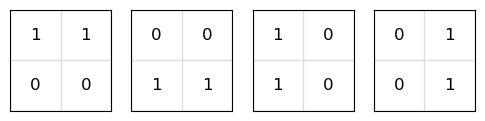
\includegraphics[height=0.1\linewidth]{Images/afficheur_digital_2}
			\label{fig:afficheur_digital_2}
		\end{figure}
		
		On notera $X \in \mathcal{M}_{4,4}(\R)$ la matrice centrée construite par empilement vertical des aplatissements (dans le sens de lecture de gauche vers la droite, du haut vers le bas) des matrices associées aux différents symboles.
		
		On donne les valeurs propres et les vecteurs propres associés de la matrice de covariance des colonnes de X:
		
		\begin{equation*}
			\lambda = \begin{pmatrix}
				1/2 & 1/2 & 0 & 0
			\end{pmatrix}
		\end{equation*}
		
		\begin{equation*}
			\begin{aligned}
				u_1 &= \begin{pmatrix} -\sqrt{2}/2 & 0 & 0 & \sqrt{2}/2 \end{pmatrix}^T \\
				u_2 &= \begin{pmatrix} 0 & \sqrt{2}/2 & -\sqrt{2}/2 & 0 \end{pmatrix}^T \\
				u_3 &= \begin{pmatrix} 0 & -\sqrt{2}/2 & -\sqrt{2}/2 & 0 \end{pmatrix}^T \\
				u_4 &= \begin{pmatrix} -\sqrt{2}/2 & 0 & 0 & -\sqrt{2}/2\end{pmatrix}^T
			\end{aligned}	
		\end{equation*}
		
		\begin{enumerate}
			\item Calculer une image moyenne.
			\item Calculer la matrice $X$ des observations.
			\item Calculer le score $Z$ du symbole \textit{gauche} par projection sur les 2 premières composantes principales.
			\item Calculer le score $Z$ du symbole \textit{haut} par projection sur la première composante principale.
			\item Calculer la reconstruction $\hat{X}$ du symbole \textit{haut} par projection sur la première composante.
			\item Déduire de la question précédente l'erreur de reconstruction du symbole \textit{haut}. On souhaite ici calculer une erreur par rapport à l'image d'origine (non centrée).
			\item En se basant sur la question précédente, est ce qu'utiliser la première composante suffit à assurer une compression sans perte ? Si non, que faudrait il faire ?
		\end{enumerate}		
	\end{exercice}
	
\end{document}